\documentclass[../thesis.tex]{subfiles}
 \begin{document}

 \begin{quote}
   For the rational study of the law the blackletter man may be the man of the present, but the man of the future is the man of statistics and the master of economics. It is revolting to have no better reason for a rule of law than that so it was laid down in the time of Henry IV. It is still more revolting if the grounds upon which it was laid down have vanished long since, and the rule simply persists from blind imitation of the past.

   - Oliver Wendell Holmes, Jr., ``The Path of the Law'', 1897 \cite{holmes1897path})
 \end{quote}
 
 This dissertation addresses one of the the great
 scientific, economic,
 and political challenge of our time: the design and
 regulation of
 the social and technical platforms such as the major
 commercially
 provided web services made available through the Internet.
 Its core contention is that no scholarly domain has yet
 comprehended the
 data economics driving the development and
 impact of this infrastructure well enough to predict and regulate its
 systemic impact.
 This scholarship labors to combine the necessary expertise
 in the correct mixture for progress.

\section{The problem}
 
 \citet{lessig2009code} has argued that cyberspace is regulated
 in four modalities: technical infrastructure, social norms,
 the law, and the market.
 Each modality has its corresponding fields of academic inquiry.
 The construction of technical infrastructure is guided
 by principles from
 electrical engineering, computer science, and statistics.
 Social norms are studied in philosophy and sociology.
 The law is both a practice and the study
 of statutes and judgements.
 Market institutions are design according to principles
 of economics.

 It would be convenient for scholars if these domains were
 as distinct from each other in practice as they are in
 theory.
 Of course, they are not, and so each branch of scholarship
 is partial and inadequate to the task of managing the Internet.
 Thoughtful leadership of technical infrastructure now comes
 primarily from the corporate leadership of private entities
 that are not tied to the academic traditions that tie down
 the institutions of public expertise.
 Since what is beyond public understanding is beyond democratic
 legal rule, the status quo is that these corporations are only
 weakly governed by law and social norms.
 This has created a public crisis
 and an opportunity for
 scientific advance \cite{benthall2016philosophy}.
 
 \section{The form of solution}

 The challenge is to construct a solution to this problem.
 What would such a scientific theory of information
 infrastructure need to be, to suffice?
 It must develop a new formal theory of strategic information
 flow and demonstrate its applicability across and
 at the intersection of all four regulatory modalities.
 This is what this dissertation does (See Figure 1.1).
 % \ref{fig:outline}
 
 \begin{figure}
  \begin{center}
  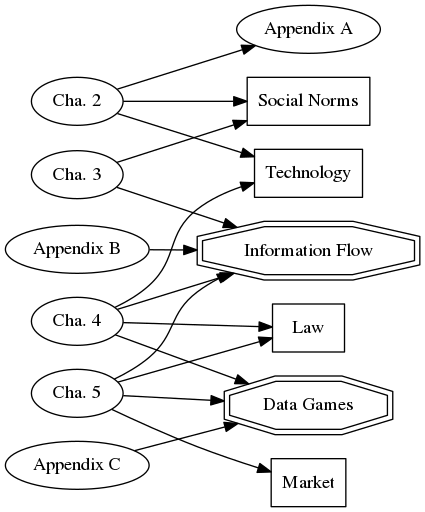
\includegraphics{chapters/outline.eps}
  \label{fig:outline}
  \end{center}
\caption[Graphical outline of this dissertation]{
  A graphical outline of the dissertation.
  Boxed components are the four modalities of
  the regulation of cyberspace.
  Round components refer to chapters and appendices
  of this document.
  Octagonal components refer to formal constructs.
  Taken as a whole, the dissertation argues that
  these formal constructs constitute scientific
  progress towards an understanding of strategic
  data flow that is applicable across all four
  modalities.
  }
\end{figure}
 
 \subsection{Social norms and technical architecture}

 A priori, we know that at the very least a solution must be
 consistent with the mathematical foundations of
 electrical engineering, computer science, and statistics.
 These are robust and objective truths that are proven
 by scientific practice and everyday experience.
 Formal, mathematical specification is a prerequisite
 to technical design, and we won't shy away from this
 desideratum.

 We also know that our theory must be sensitive to social
 norms.
 Herein lies the first major obstacle: the
 sociologists, anthropologists, and philosophers who best
 understand social norms are often alienated by
 mathematical formalism.
 Most (though not all) would reject the possibility that
 norms may be understood well enough by technologists
 that the latter could be adequately responsive to them.

 But not all.
 Contextual integrity (CI) is a social theory of privacy norms
 that has been actively offered to computer scientists
 as a guide to technical design.
 This work at the intersection of social theory and
 privacy engineering is the subject of 
 Chapter \ref{chapter:CI-through-CS} of this
 dissertation, ``Contextual Integrity through the Lens of Computer Science'', co-authored by myself, Seda G{\"u}rses and
 Helen Nissenbaum \cite{benthall2017contextual}.
 It is a survey of computer science papers that have been
 inspired by CI.
 We compare the original social theory with its technical projection, and identify both opportunities for contextual integrity to be made more technically actionable and calls to action for computer scientists to better accomodate social processes and meaning.

 Contextual integrity, which is described in detail in
 Section \ref{CI2.1}, defines privacy as contextually
 appropriate information flow.
 It envisions a social world differentiated into multiple
 social contexts or spheres, each with well-defined
 roles, purposes, and meanings of information.
 In Chapter \ref{chapter:CI-through-CS}, we discover that
 computer scientists see the world differently.
 They design infrastructure for a messy reality in which
 information crosses contextual boundaries.

 In short, technical and social platforms are not well
 regulated by social norms because they exist outside
 of our shared understanding of social contexts.
 Chapter \ref{chapter:bridge} briefly assesses these conclusions
 and identifies the  heart of the problem:
 the ambiguity inherent in our socially shared
 understanding of \textit{information flow}.
 That understanding is based on a flawed ontology
 in which data's meaning is contained within it.
 This is not the case \cite{horvitz2015data};
 the meaning of information depends on the context,
 or contexts, in which it flows.
 Effective design and regulation of information
 infrastructure requires a scientific
 definition of information flow that addresses this
 fact precisely.
 
 \subsection{Law, technical architecture and situated information law}

 Such a definition of information flow is provided in
 Chapter \ref{chapter:origin-privacy},
 ``Origin Privacy: Causality and Data Protection'', originally
 written as a technical report
 with Michael Tschantz and Anupam Datta. 
 It is targetted at another dyad in the regulation of information
 infrastructure: the interaction between technical architecture
 and information law.

 This chapter builds on previous work in the automation of
 regulatory compliance.
 Businesses and other organizations are motivated to comply
 with privacy policies even as their information
 processing systems get more complex \cite{barth2007privacy}
 \cite{deyoung2010experiences} \cite{sen2014bootstrapping}.
 This business interest has driven scholarhsip in the
 mathematical formulation and implementation of law
 in computer science.

 The concept of information implicit in privacy policies
 has ambiguities that are similar to those identified
 in Chapter \ref{chapter:bridge}: information is sometimes
 restricted based on its topic, and other times restricted
 based on its origin.
 What theory of information can capture how information
 flows from source to destination with meanings that depend
 on context?

 Building on \citet{dretske1981knowledge}
 and \citet{pearl2009causality}, we posit a definition
 of information flow as a causal flow within a greater
 context of causally structure probabilistic events.
 The context provides each event with
 \textit{nomic associations}, or law-like, regular
 correspondences with other events in the causal system.
 The nomic associations are what make information useful
 for inference and thereby meaningful.

 Chapter \ref{chapter:origin-privacy} develops this
 theoretical understanding of situated information flow as a
 tool for understanding the security of information processing
 systems.
 It develops the Embedded Causal System (ECS) model,
 a generic way of modeling an information processing system
 embedded in an environment.
 We use this model to define variations of well-known
 security properties such as noninterference and semantic
 security in terms of Pearlian causation,
 and prove sufficient conditions for systems to have these
 properties.
 We consider a new class of security properties based on
 Origin Privacy, the principle that a system designer
 must control information flow based on that information's
 origin.
 We further extend this model to the GDPR's regulation of
 biometric data and differential privacy.
 We also introduce a game theoretic variation on the model
 which relates the causal security properties to the tactical
 and strategic presence of an attacker.
 Developing this style of strategic modeling is the
 project of Chapter \ref{chapter:games-and-rules}.

 \subsection{Information law and data economics}

 It is just a fact that most information infrastructure
 today is developed by industry, military, or both.
 No sufficient theory of infrastructure design can
 deny that there is a strategic aspect to its
 creation and use.
 Though there is a tradition of economics literature
 on the business of information goods
\cite{shapiro1998information}
\cite{varian2001economics} \cite{acquisti2016economics},
this scholarship has not captured the economics of data flow
and reuse
in a way that is commensurable with technical design and
available to legal scholars for regulatory design.
Chapter \ref{chapter:games-and-rules} fills this gap.

 Chapter \ref{chapter:games-and-rules} works with the
 definition of situated information flow introduced in
 Chapter \ref{chapter:origin-privacy} and builds
 it into a framework for economic mechanism design
 (detailed in Appendix \ref{appendix:maid})
 using the Multi-Agent Influence Diagrams
 of \citet{koller2003multi}.
 This framework is the basis for a formal method for
 determining the value of information flow within a
 \textbf{data game}.

 This framework can capture well-understood economic
 contexts such as principal-agent contracts and
 price differentiation.
 It can also support the modeling and analysis of
 newly introduced economic situations, such as the provision
 of personalized expert services and the
 value of the cross-context use of personal data.
 The model of cross-context use of personal data
 reveals that when firms trade in the personal data
 of their users, they can benefit at their user's expense.
 Because the user is not a party to this transaction,
 effects on their welfare may be considered a market externality,
 which invites the discussion of what form of
 regulation is appropriate to fix the market deficiency.

 What this chapter demonstrates is that information
 is not, contrary to many traditional economic models,
 a kind of good that is consumed.
 Rather, information is a strategic resource, something
 that changes the very nature of the game played by
 economic actors.
 A thorough study of data economics through the
 modeling, simulation, and empirical analysis of
 data games may be the scholarly lens needed to
 understand how technical architecture, social norms,
 law, and the market interact and resolve in equilibrium.

 Chaper \ref{chapter:conclusion} concludes this dissertation
 with a discussion of future work.
 
\end{document}
